\section[Script to Agent]{Script to Agent: From code to deployment}

This section describes the process of deploying a DSL script, from to code, to a functioning agent enforcing rules and generating reports.

First the 

\begin{figure}[h]
    \centering
    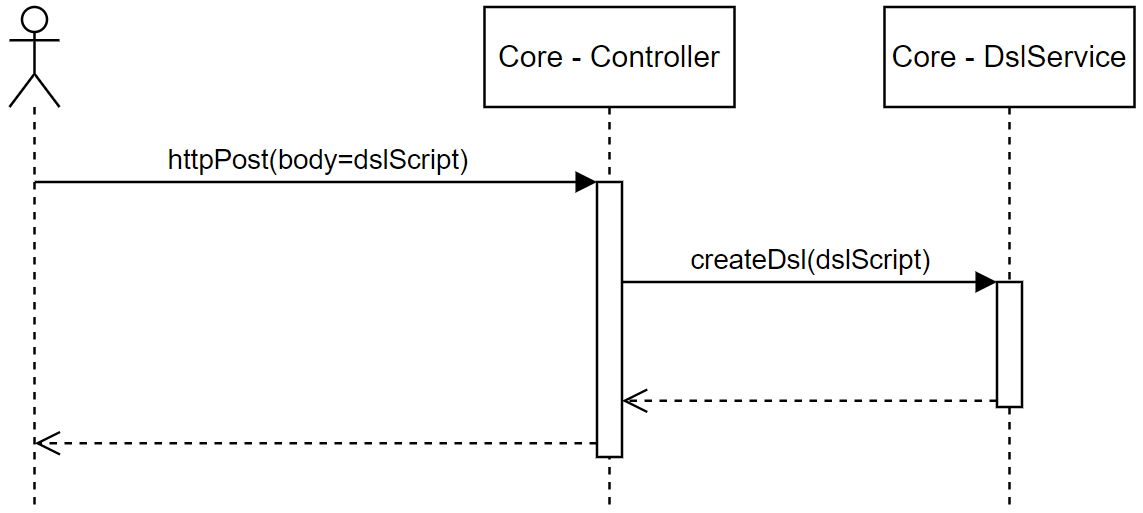
\includegraphics[width=130mm, keepaspectratio]{seq0.png}
    \caption{Complex architecture plan}
    \label{fig:comp_arch}
\end{figure}

script is uploaded on uid
compilation starts
    pull script
    prepare file
    gradle build
    mention: caching, how the builder image is created
    explain build health check and cleaing cycle
once compiled it can be started
process of starting:    
    read script to memory, execute it to get the wh conf data
    get tls cert
    create k8s resources: deployment service, whsconf, crb
    explain agent health check
    explain rollback
agent starts, agent downloads script with curl
    explain why is it good to precompile script
    dynamically link compiled jar -cp ; custom class loader
    use reflection to find the getServer method
    configuring router